\documentclass[a4paper]{report}
\usepackage[english]{babel}
\usepackage[utf8]{inputenc}
\usepackage{graphicx}
\usepackage{enumitem}
\usepackage{multirow}
\usepackage{listings}
\usepackage{biblatex}
\usepackage{todonotes}
\addbibresource{references.bib}
\graphicspath{ {./images/} }

\title{Bachelor Thesis}
\author{Emil Valbak Hermansen}
\date{October 2020}

\begin{document}
\listoftodos
\begin{abstract}
    This document will contain different latex syntax examples which can be used for the bachelor thesis. 
\end{abstract}

\maketitle
\tableofcontents

\chapter{Graphics}
\todo{Add better graphics}
    This will contain examples of how to handle graphics

    \section{Image caption}
        \begin{figure}[h]
            \caption{A picture of a monkey}
            \centering
              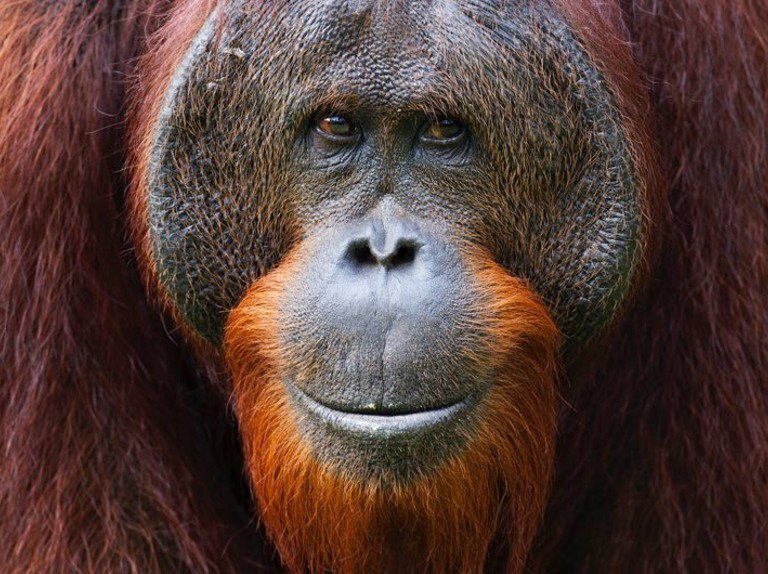
\includegraphics[width=0.5\textwidth]{abe.jpg}
              \label{fig:monkey_cap_upper}
        \end{figure}

        \begin{figure}[h]
            \centering
            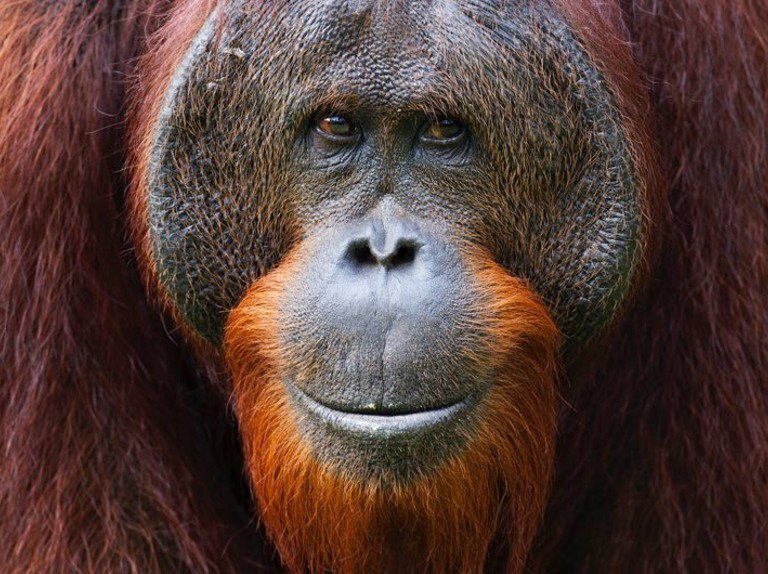
\includegraphics[width=0.5\textwidth]{abe.jpg}
            \caption{A picture of a monkey}
            \label{fig:monkey_cap_bottom}
        \end{figure}

        \begin{figure}[h]
            \caption{Comparison of monkey from figure \ref{fig:monkey_cap_bottom} and \ref{fig:monkey_cap_upper}}
            \centering
            \label{fig:comparison_of_monkeys}
            \begin{minipage}[b]{0.4\textwidth}
                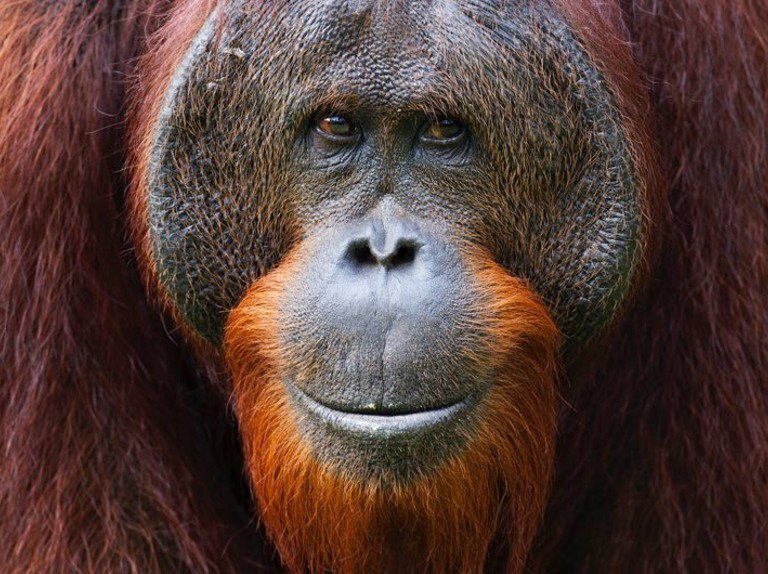
\includegraphics[width=\textwidth]{abe.jpg}
                \caption{Monkey one}
              \end{minipage}
              \hfill
              \begin{minipage}[b]{0.4\textwidth}
                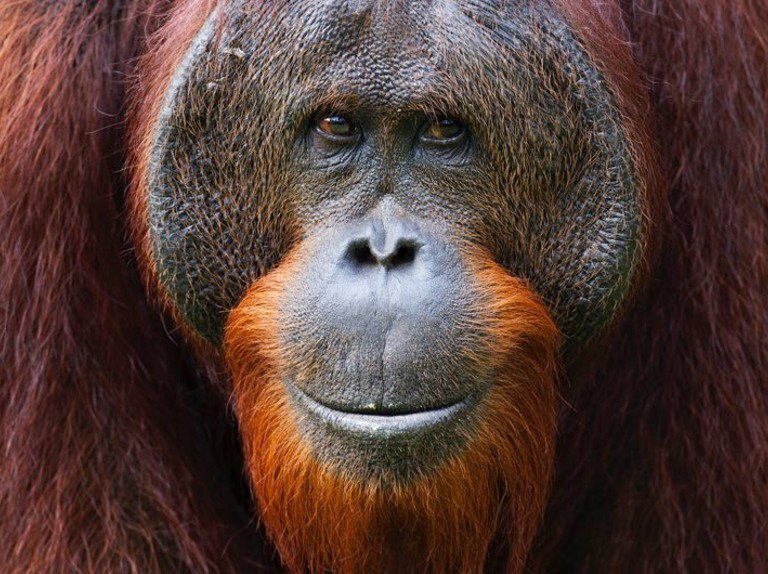
\includegraphics[width=\textwidth]{abe.jpg}
                \caption{Monkey two}
              \end{minipage}
        \end{figure}

\chapter{Reference to image}
As seen in figure \ref{fig:monkey_cap_bottom}, the monkey is very handsome
\chapter{Reference to page containing the image}
This handsome monkey can be found on page \pageref{fig:comparison_of-monkeys}
\chapter{Section, subsection, subsubsection, paragraph, subparagraph}
    \section{This is a numbered section}
    \section*{This is a non-numbered section}
    
\chapter{Lists}
\todo{Add more items to lists}
    \section{Bullet points}
        \begin{itemize}
            \item[--] This is a normal bullet point
            \item[$-$] Slighty different dash
            \item[$\ast$] Asterisk bullet point
        \end{itemize}
    \section{Numbered lists}
        \subsection{Numbers} 
            \begin{enumerate}[label=\arabic*)]
                \item One
                \item Two
                \item Three
            \end{enumerate}
        \subsection{Roman numerals} 
            \begin{enumerate}[label=(\roman*)]
                \item One
                \item Two
                \item Three
            \end{enumerate}
            
        \subsection{Letters} 
            \begin{enumerate}[label=\alph*)]
                \item One
                \item Two
                \item Three
            \end{enumerate}
            

\chapter{Table with multiple columns}

\section{Various horizontal alignments in columns (left, right, centered), descriptions and labels, reference}
    In this section we will look a tables, and table \ref{table:orangutan_population_horizontal_alignments} shows population of orangutan species\cite{sen2005cute}
    \begin{table}[!h]
        \begin{tabular}{lll}
            \hline
            \multicolumn{1}{|l|}{\textbf{Scientific name}} & \multicolumn{1}{c|}{\textbf{Common name}} & \multicolumn{1}{r|}{\textbf{Estimated number}} \\ \hline
            \multicolumn{1}{|l|}{Pongo abelii}             & \multicolumn{1}{c|}{Sumatran orangutan}   & \multicolumn{1}{r|}{14,613}           \\ \hline
            \multicolumn{1}{|l|}{Pongo tapanuliensis}      & \multicolumn{1}{c|}{Tapanuli orangutan}   & \multicolumn{1}{r|}{\textless{}800}   \\ \hline
            \multicolumn{1}{|l|}{Pongo pygmaeus}           & \multicolumn{1}{c|}{Bornean orangutan}    & \multicolumn{1}{r|}{\textgreater{}53,960}   \\ \hline
        \end{tabular}     
        \caption{Population of different orangutan species}
        \label{table:orangutan_population_horizontal_alignments}
    \end{table}
    
\section{Cell spanning multiple columns}
    \begin{tabular}{|l|l|l|}
        \hline
        first column & second column & third column \\
        \hline
        \multicolumn{3}{|c|}{Cell spanning three columns} \\
        \hline
    \end{tabular}

\section{Vertical alignment in multi-line cells}
    \begin{table}[!h]
          \begin{tabular}{|c|c|c|} \hline
            Column 1 & Column 2 & Column 3 \\ \hline
            \multirow{2}{*}{Double row} & Upper 2 & Upper 3 \\ 
            & Lower 2 & Lower 3 \\ \hline             
          \end{tabular}
        \label{tab:multirow}
      \end{table}

    
\chapter{Code listing}\cite{sen2005cute}
    \begin{lstlisting}[language=Python]
        import numpy as np
            
        def incmatrix(genl1,genl2):
            m = len(genl1)
            n = len(genl2)
            M = None #to become the incidence matrix
            VT = np.zeros((n*m,1), int)  #dummy variable
            
            #compute the bitwise xor matrix
            M1 = bitxormatrix(genl1)
            M2 = np.triu(bitxormatrix(genl2),1) 
        
            for i in range(m-1):
                for j in range(i+1, m):
                    [r,c] = np.where(M2 == M1[i,j])
                    for k in range(len(r)):
                        VT[(i)*n + r[k]] = 1;
                        VT[(i)*n + c[k]] = 1;
                        VT[(j)*n + r[k]] = 1;
                        VT[(j)*n + c[k]] = 1;
                        
                        if M is None:
                            M = np.copy(VT)
                        else:
                            M = np.concatenate((M, VT), 1)
                        
                        VT = np.zeros((n*m,1), int)
            
            return M
    \end{lstlisting}

\chapter{Bibliography with book, article and internet link}
Citing examples:
Book Here\cite{dirac} 
Article here\cite{einstein}  
Internet link here\cite{orangutanwiki}  

\chapter{Some kind of todo notes}
\printbibliography

\end{document}
